\chapter{Scrum process supplementary materials}
%TC:ignore
The appendix discusses some of the additional material to show the process of scrum used as the methodology of choice.
Below is a collection of user-stories throughout the sprints.
\section{Sprint burndown charts}
\begin{figure}[H]
  \centering
  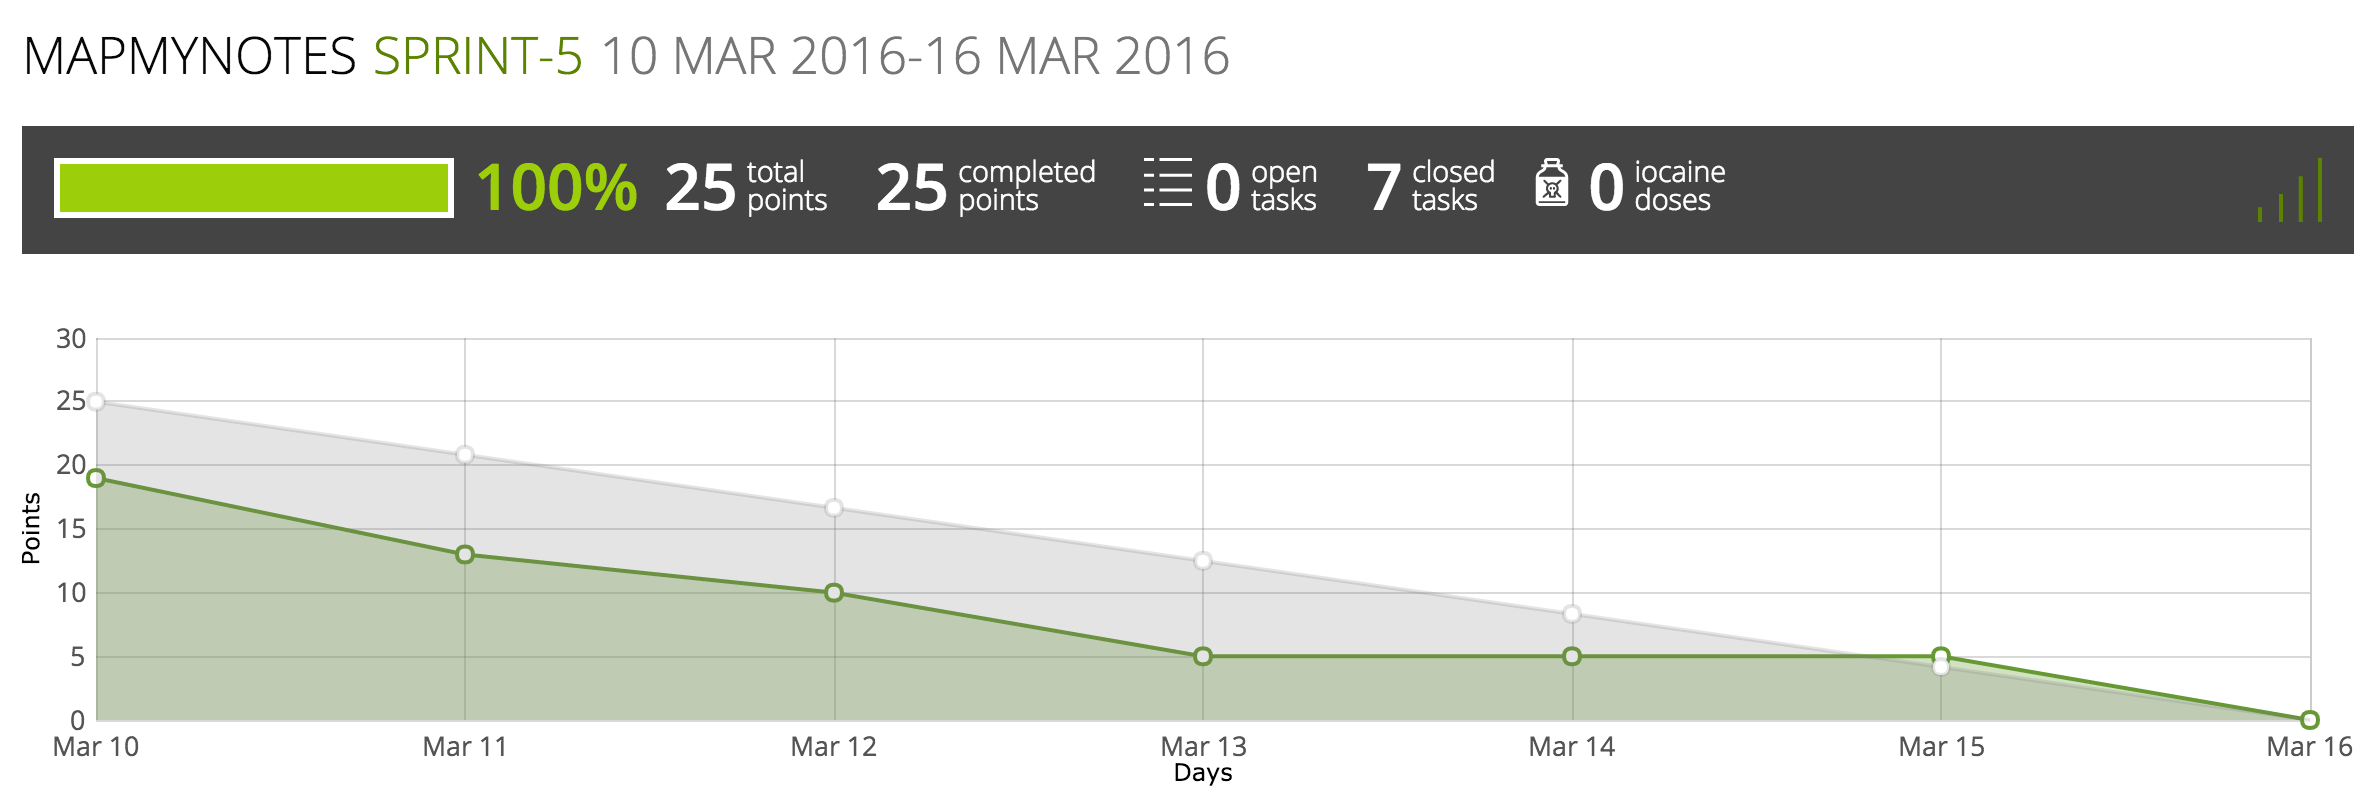
\includegraphics[scale=0.35]{images/sprint-5-burndown-chart}
  \caption{An example of the burndown chart for a sprint, showing areas where there may have been difficulty.}
  \label{fig:sprint-burndown}

\end{figure}

\section{Overall burndown chart}
\begin{figure}[H]
  \centering
  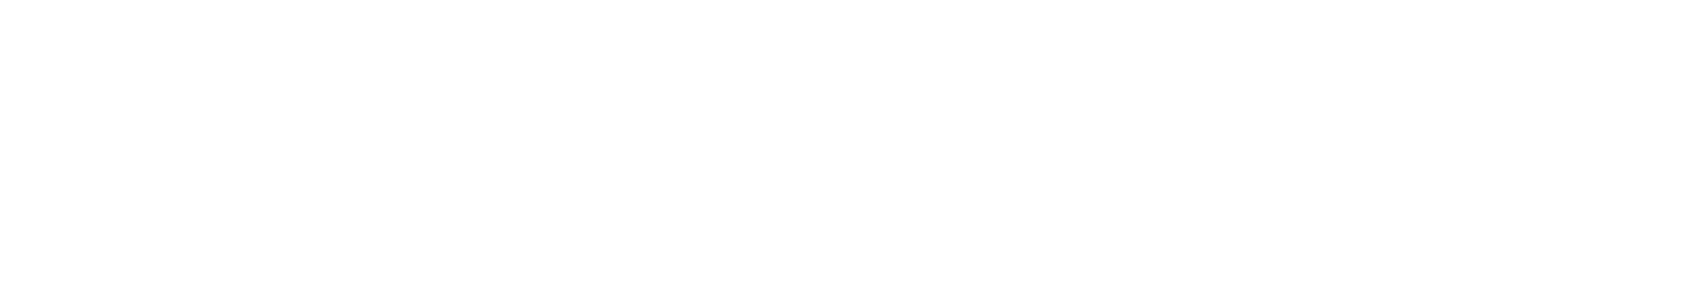
\includegraphics[scale=0.5]{images/overall-burndown}
  \caption{The overall burndown of the sprints during the development period. This clearly shows a consistent work flow up until more knowledge of the project was achieved, going below the expectation line.}
  \label{fig:overall_burndown}
\end{figure}

\begin{table}[h!]
\centering
\begin{tabular}{|p{1cm} p{10cm} p{1cm} p{1cm}|}
   \hline
 Id & User story & Sprint & Story points \\ [0.5ex]
 \hline\hline
 1 & As a user I want to be able to upload an image of a set of notes so that I can see my note in the application & 2	& 10 \\
 2 & As a user I want to be able to tag my notes so that  all my notes are under the correct module	& 4	 & 5 \\
 3&As a user I want to be able to add information about the notes so that I can reference them in the future&4&15 \\
 4&As a user I want to be able to save a note, so that I can find it again later&3&10 \\
 5&As a user I want to be able to search for a given module, so that I can find all notes for that module&7&8 \\
 6&As a user I want to be able to sign in via google sign in&5&15 \\
 7&As a user I want to use Tesseract OCR so that I can identify characters&1&15 \\
 8&As a user I want to be able to view the application on a website&2&5 \\
 9&As the customer I want to see the image being binarised properly&2&10 \\
 10&As a developer I need to train my handwriting, so that Tesseract can recognise my handwriting&10&n/a \\
 11&As a user I want to be able to edit the meta data, so that I can update it in light of a change&5&5 \\
 12&As a user I want to be able to remove a note incase I do not want it to appear&5&5 \\
 13&As a developer I want to the website to have good styling&4&8 \\
 14&As a developer I want to integrate tesseract into the application, so it can read information from a note&8&8 \\
 15&As a user I want to be able to view all the notes I have as a user so I can easily find all of them again&6&3 \\
 16&As a user I want to view a list of events on the homepage from my calendar, so I can see recent events&6&15 \\
 17&As a user I want to be able to save the URL in the calendars event&7&10 \\
 18&As a user I want to be able to tag the title of the lecture, so that I can know which one it is.&6&5 \\
 19&As a user, when I authorise I want to show my email address and remove the authorise button, so I know I have signed in&6&3 \\
 20&As a developer I want to be able to get the date taken from EXIF data, to show information about a note&7&8 \\
 21&As a user I want to be able to edit the date and update my calendar&9&8 \\
 22&As a developer I want to be able to associate a note with a user&7&5 \\
 23&As a user, I want to be able to have automated suggestion of meta data from the image, so that I can know what to tag.&8&5 \\
 24&As a user, I want to be able to logout, so that I can close my session&8&5 \\
 25&As a user I want to be able to click Tesseract Items, so that it's easier for me to put in the fields.&9&10 \\
 26&As a user I want to be able to edit and save to reoccurring events&10&10 \\
 \hline
 \end{tabular}
 \caption{A table showing the user stories identified throughout the project, along with the sprint in which they were implemented and associated story points}
\end{table}
%TC:endignore
